% Dit werk is gelicenseerd onder de licentie Creative Commons Naamsvermelding-GelijkDelen 4.0 Internationaal. Ga naar http://creativecommons.org/licenses/by-sa/4.0/ om een kopie van de licentie te kunnen lezen.
\documentclass[11pt,twoside]{article}

\usepackage[margin=2.5cm]{geometry}     % Marges instellen
\usepackage[dutch]{babel}               % Voor nederlandstalige hyphenatie (woordsplitsing)
\usepackage{graphicx}         			% Om figuren te kunnen verwerken
\usepackage[utf8]{inputenc}             % Om niet ascii karakters rechtstreeks te kunnen typen
\usepackage{parskip}                    % Om paragrafen met een verticale spatie ipv horizontaal te starten
\usepackage{listings}					% Om code weer te geven
\usepackage{courier}
\usepackage{textcomp}
\usepackage[pdftex,                     % Om hyperlinks en metadata te hebben in het pdfdocument.
			plainpages=false,
            pdfauthor={Brecht Baeten},
            pdftitle={Inleiding to Python}]{hyperref}

\lstset{language=Python,
        basicstyle=\footnotesize\ttfamily,
        tabsize=4,
        breaklines=true,
        showstringspaces=false,
        upquote=true}

\title{Inleiding tot Python}
\author{Brecht Baeten}

\begin{document}

	\maketitle

	\section{Wat is Python?}
Python is een open source programmeer taal. Voor ingenieurstoepassingen of wetenschappelijke projecten is Python interessant aangezien er een aantal Python modules bestaan die hier specifiek op gericht zijn. Deze modules maken het beheren van data of uitvoeren van complexe wiskundige algoritmes zeer eenvoudig, vandaar de populariteit. Python werkt volledig object georiënteerd, dit laat toe efficiente en leesbare code te schrijven. Het schijven van leesbare code is één van de hoekstenen van Python aangezien code veel vaker gelezen wordt dan geschreven. Python code hoeft ook niet gecompileerd te worden (althans niet door de gebruiker). Python is een geïnterpreteerde programmeertaal wat inhoudt dat code rechtstreeks uitgevoerd kan worden zonder eerst te compileren. Een ander groot voordeel van Python boven bijvoorbeeld Matlab is dat het gratis is! Iedereen, wetenschappers, studenten, particulieren, grote of kleine bedrijven kan Python gratis downloaden en gebruiken. In veel Linux distributies word Python standaard meegeleverd wat zelfs de installatie overbodig maakt.

Een nadeel van Python ten opzichte van Matlab is dat de verschillende beschikbare IDE's (Integrated Development Environments) veel minder vloeiend en gebruiksvriendelijk zijn dan de bekende Matlab interface. Dit is echter slechts een klein nadeel ten opzichte van de vele voordelen van Python.

De broncode van deze tekst alsook alle voorbeelden kunnen worden gedownload via \url{https://github.com/BrechtBa/inleiding-tot-python/}.

	\section{Installatie in Windows}
Alle nog ondersteunde versies van Python kunnen worden gedownload via \url{https://www.python.org/downloads/}. Hier vind je de broncode en installer executables voor verschillende platformen. Downloaden, uitvoeren en klaar. Het is wel aan te randen om niet de nieuwste versie te installeren aangezien verschillende modules een tijdje nodig hebben om hun code aan te passen naar een nieuwe versie. Tijdens de installatie is het interessant om Python aan je Windows search path toe te voegen, zo kan je python steeds van in een command line interface openen. Het is ook interessant om de installatie locatie te veranderen naar bijvoorbeeld  "\textsf{C://python34}".

Je kan nu al Python starten door op python.exe te klikken. Er opent een console waarin je python commando's kan invoeren (zie Figuur \ref{fig:Python34}). Typ hier bijvoorbeeld:
\begin{lstlisting}
print('Hello World!')
\end{lstlisting}

Druk op enter en je hebt je eerste python commando uitgevoerd.
\begin{figure}[ht]
	\centering
	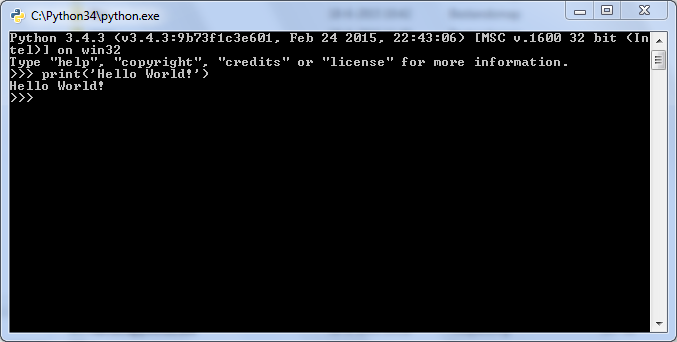
\includegraphics[scale=0.5]{fig/Python34}
	\caption{Python console met eerste commando}
	\label{fig:Python34}
\end{figure}

Python code kan opgeslagen worden in eenvoudige tekst bestanden met de extentie "\textsf{.py}". Om deze te schrijven is een goede text editor met syntax highlighting aan te raden. In Windows is \emph{notepad++} een goed, open source alternatief met syntax highlighting voor Python en een groot aantal andere talen ingebouwd. \emph{notepad++} kan worden gedownload via \url{https://notepad-plus-plus.org/download/}.

Omdat Python vanuit een command line interface zal worden aangeroepen is het interessant om een deftige console te installeren. \emph{ConEmu} is een open source console emulator met gelijkenissen aan \emph{bash} in Linux. Deze is te downloaden vanaf \url{http://sourceforge.net/projects/conemu/files/latest/download}. Simpelweg downloaden, unzippen in een folder naar keuze en klaar. De standaard \emph{cmd} console kan echter ook gebruikt worden.

 	\section{Scripts}
Omdat het telkens opnieuw invoeren van commando's achter elkaar niet zo praktisch is, is het interessant om een reeks commando's op te slaan in een script en dit uit te voeren. Open een teksteditor en typ "\lstinline{print('Hello World!')}"\ en sla het bestand op als \textsf{hello\_world.py}. Om het bestand uit te voeren open je een console, navigeer naar de locatie waar je het bestand hebt opgeslagen, typ "\lstinline[language=bash]{python hello_world.py}"\ en druk op enter. Het resultaat is hetzelfde als daarnet.

Python heeft een aantal interessante ingebouwde variabele types. Open een nieuw bestand, typ onderstaande commando's en sla het op als \textsf{variables.py}.
\lstinputlisting{examples/variables.py}

Voer het script ditmaal uit met het commando "\lstinline[language=bash]{python -i variables.py}". De "\lstinline[language=bash]{-i}"\ zorgt ervoor dat python na het uitvoeren van alle commando's in het script naar de interactieve console gaat. Alle reeds gedefinieerde variabelen zijn nu ook beschikbaar in de console. Typ bijvoorbeeld:
\begin{lstlisting}
E[3]
\end{lstlisting}
of:
\begin{lstlisting}
A+B
\end{lstlisting}
Door "\lstinline{Ctrl+Z}"\ in te geven kan je Python afsluiten en terugkeren naar de command line interface.

Zoals te merken in het voorgaande voorbeeld is Python zeer flexibel met data types. Zo kunnen een \emph{Integer} en een \emph{Float} met elkaar opgeteld worden en kan een \emph{List} elementen met verschillende datatypes bevatten. Een zeer interessant data type is het \emph{Dictionary} of \emph{dict}. Hierin kunnen key / value paren worden opgeslagen en terug opgeroepen. Zowat elke Python variabele kan een \emph{Dictionary} key zijn wat dit type zeer flexibel maakt. Het is gewenst om even in te gaan op de manier van indexeren in Python. Een Python \emph{List} start bij index 0. Het laatste element kan je oproepen met de index -1, het voorlaatste met index -2, enz. Je kan een deel van de lijst opvragen met behulp van de "\lstinline{:}"\ operator, de subset loopt dan van de index voor de "\lstinline{:}"\ tot (niet tot en met) de index erna. Indien er geen index voor of achter de "\lstinline{:}"\ staat zal de subset starten of eindigen bij respectievelijk het eerste of het laatste element.

Er moet even aandacht besteed worden aan de manier waarop variabelen in Python gebruikt worden. In Python zijn variabelen slechts namen die naar een bepaalde waarde verwijzen. Wanneer een variabele toegewezen wordt, wordt enkel de referentie naar de waarde toegewezen. In het voorbeeld hierboven zullen "\lstinline{print(F)}"\ en "\lstinline{print(G)}"\ hetzelfde resultaat geven. Hierboven wordt "\lstinline{H}"\ echter gedefinieerd als een nieuwe \emph{Dictionary} met dezelfde waarden als "\lstinline{F}". De commando's "\lstinline{print(F)}"\ en "\lstinline{print(H)}"\ zullen dus een verschillend resultaat hebben.

Echt programmeren begint pas bij maken van lussen en voorwaarden: flow control. In python is dit zeer eenvoudig met behulp van "\lstinline{for}"\ lussen of "\lstinline{if else}"\ structuren:
\lstinputlisting{examples/flow_control.py}

In Python moet elk flow control element eindigen met een ":". De code binnen het element moet een tab inspringen. Dit zorgt voor een zekere leesbaarheid in de code. De "\lstinline{range(10)}"\ functie in de "\lstinline{for}"\ lus maakt een \emph{List} met waarden van 0 tot en met 9. De "\lstinline{.format(i)}"\ functie formatteert zijn inhoud op de plaats van de accolade's in de voorafgaande string. De format functie is eigenlijk een methode van het \emph{String} datatype en geeft een hele reeks formatteer opties. Even zoeken op het net leert je heel veel over zulke ingebouwde functies.

Je kan over zowat elk datatype itereren. Een lus over een dictionary kan bijvoorbeeld op verschillende manieren. Ook itereren over verschillende variablen tegelijk is eenvoudig met de "\lstinline{zip()}"\ functie. Indien je itereert over een \emph{List} en de index van de variabelen wil gebruiken kan je de functie "\lstinline{enumerate()}"\ gebruiken:
\lstinputlisting{examples/flow_control_advanced.py}

Een set commando's die vaak op dezelfde manier gebruikt worden kan je groeperen in een functie. Een functie definieer je met het "\lstinline{def}"\ keyword, gevolgd door de functie naam, de argument namen tussen haakjes en een dubbelpunt. Argumenten kunnen verplicht of optioneel zijn. voor optionele argumenten moet een default waarde opgegeven worden in de functie definitie. Alle verplichte argumenten moeten ook voor de optionle komen in de functie definitie. Wanneer een functie veel optionele argumenten heeft is het gemakkellijk om deze via naam=waarde paren op te geven, de volgorde is dan niet meer van belang:
\lstinputlisting{examples/functions.py}

Variabelen die binnen een functie gedefinieerd zijn bestaan ook enkel in de functie namespace. Bovenstaande code geeft dus een error omdat \lstinline{val} enkel in de functie namespace gedefinieerd is, niet in de globale namespace. Functies kunnen wel gebruik maken van variabelen in de globale namespace maar niet omgekeerd. Wanneer de bovenstaande code runt krijg je dan ook de volgende foutmelding:
\begin{lstlisting}[language=bash]
Traceback (most recent call last):
  File "C:\examples\functions.py", line 10, in <module>
    print(val)
NameError: name 'val' is not defined
\end{lstlisting}

	\section{NumPy, SciPy en Matplotlib} 
Er bestaan enorm veel modules waarin specifieke functie gedefinieerd zijn voor gebruik in Python. Drie voor Ingenieurs interessante modules zijn \emph{NumPy}, een lineair algebra module, \emph{SciPy}, een algemeen wetenschappelijke wiskunde module en \emph{Matplotlib}, een module voor het maken van figuren van hoge kwaliteit. Windows installers kunnen worden gedownload via \url{http://sourceforge.net/projects/numpy/files/NumPy/}, \url{http://sourceforge.net/projects/scipy/files/scipy/} en \url{http://matplotlib.org/downloads.html}. Kies de binary die overeenkomt met jou systeem architectuur en python versie, downloaden en installeren. De meeste modules lopen steeds één versie achter op de laatste Python release, het kan dus interessant zijn om een iets oudere versie van Python te installeren.

Om een module te kunnen gebruiken in een script moet deze eerst geïmporteerd worden. Dit gebeurt met een "\lstinline{import}"\ statement en kan op verschillende manieren. In Python blijft elke geïmporteerde module zijn eigen namespace behouden. Je kan dus de \lstinline{linspace} funtie uit \emph{NumPy} aanroepen als "\lstinline{numpy.linspace(...)}". Om de notatie wat te verkorten kan je een module importeren onder een zelf gekozen naam met "\lstinline{import ... as ...}"\ zoals aangegeven in het voorbeeld hieronder. Voor meer info over \emph{NumPy} of \emph{SciPy} wordt verwezen naar de online documentatie op \url{http://docs.scipy.org/doc/numpy/} en \url{http://docs.scipy.org/doc/scipy/reference/}

\emph{Matplotlib} kan \LaTeX\ gebruiken om tekst weer te geven, dit kan permanent gedaan worden door de 'rc' parameters aan te passen in het \textsf{matplotlibrc} bestand of deze in het script zelf aan te passen zoals hieronder aangegeven. De grootte van de figuur wordt in inch opgegeven vandaar een correctiefactor naar centimeter. Met behulp van de "\lstinline{savefig}"\ functie wordt de figuur opgeslagen als pdf (Figuur \ref{fig:sinus_cosinus}). Een zeer groot aantal voorbeelden van \emph{Matplotlib} figuren en de code gebruikt om ze te maken is terug te vinden op \url{http://matplotlib.org/gallery.html}.
\lstinputlisting{examples/numpy_scipy_matplotlib.py}

\begin{figure}[ht]
	\centering
	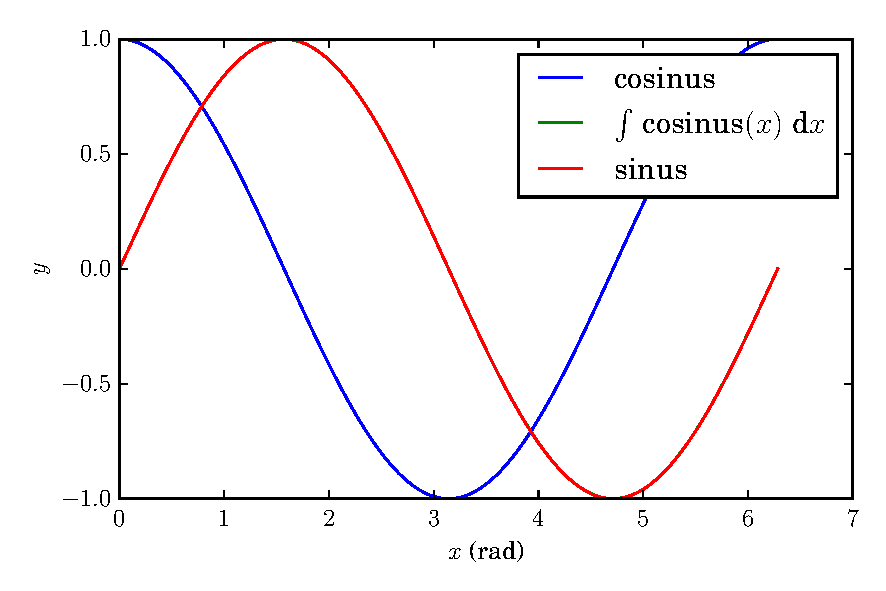
\includegraphics[scale=0.5]{examples/sinus_cosinus}
	\caption{Matplotlib voorbeeld}
	\label{fig:sinus_cosinus}
\end{figure}

	\section{Object georiënteerd} 
Een grote sterkte van Python is de zeer grote object gerichtheid van de programeertaal. Zowat alles in Python is een object met zijn methodes en kan aangepast of gebruikt worden in child klasses. Een klasse wordt in python gedefinieerd met het keyword "\lstinline{class}"\ gevolgd door de klassenaam het basis object tussen haakjes en een dubbelpunt. Opnieuw dient alles wat binnen de klasse definitie valt één tab verschoven te zijn tenopzichte van de klasse definitie. Binnen een klasse zijn er een aantal belangrijke methodes die kunnen gebruikt worden. De eerste is de "\lstinline{__init__}"\ methode. Deze wordt gebruikt om een object instance te creëren. Het eerste argument is steeds "\lstinline{self}", dit wordt gebruikt om attributen aan de instance toe te kennen, verder kunnen de argumenten op dezelfde wijze als bij functies gedefineerd worden. De "\lstinline{__}"\ voor en na de methode definitie geven aan dat deze een ingebouwde functie heeft. In het voorbeeld hieronder wordt ook de "\lstinline{__str__}"\ methode gedefinieerd die het printen van het object definieert. Telkens is "\lstinline{self}"\ het eerste argument om een referentie naar de huidige object instance te hebben.

In het voorbeeld hieronder wordt ook een \lstinline{density} methode gedefinieerd die gebruikt kan worden om de dichtheid van het gas te berekenen. Onmiddellijk na de definitie volgt de documentatie van de functie tussen drie aanhalingstekens "\lstinline{"""}". Deze wordt weergegeven indien de de "\lstinline{help()}"\ functie wordt opgeroepen, dit kan trouwens ook bij gewone functies. Het is een goede gewoonte om hier steeds te schijven wat de functie doet, wat ze returnt, wat de argumenten betekenen en welk datatype de argumenten moeten zijn. Een andere goede gewoonte is om methodes die bedoeld zijn om enkel binnen de klasse definitie te gebruiken te beginnen met een "\lstinline{_}". Op die manier is het voor een gebruiker van de klasse meteen duidelijk dat deze methode niet voor hem of haar bedoeld is. 

In de code hieronder is het gedeelte dat rechtstreeks uitgevoerd moet worden in een "\lstinline{if __name__ == '__main__':}"\ geplaatst. Dit zorgt ervoor dat deze code enkel uitgevoerd wordt als het script rechtstreeks wordt uitgevoerd. Meer hierover in de volgende sectie.
\lstinputlisting{examples/object_oriented.py}

Een belangrijk element van object georiënteerd programeren is inheritance. In Python is dit opniew zeer eenvoudig. In het voorbeeld hieronder wordt een "PerfectGas"\ klasse gedefinieerd op basis van van de eerder gemaakte "IdealGas"\ klasse. De eerste regel zorgt ervoor dat de "IdealGas"\ klasse beschikbaar is in dit script, meer hierover in Sectie \ref{sec:Eigen modules schrijven}. We kunnen nu methodes van de parent klasse herdefiniëren of nieuwe methodes toevoegen. In het voorbeeld hieronder wordt de "\lstinline{__str__}"\ methode aangepast door iets toe te voegen aan de originele methode met behulp van de "\lstinline{super}"\ functie. Merk op dat alle methodes van de parent klasse nog steeds beschikbaar zijn.
\lstinputlisting{examples/inheritance.py}
	
De bedoeling van inheritance is om zoveel mogelijk code te hergebruiken, en dus geen code dubbel te schrijven, wat moeilijk te onderhouden is.

 	\section{Eigen modules schrijven}
 	\label{sec:Eigen modules schrijven}
Wanneer een project groeit komt er een moment dat het niet meer interessant is om alle code in één file the schrijven. In Python kan dit door het project op te delen in modules en deze in een hoofd bestand te importeren en te gebruiken. Een Python module kan je definiëren door in een folder een bestand "\textsf{\_\_init\_\_.py}"\ aan te maken. In dit bestand kan je code zetten die uitgevoerd dient te worden tijdens de initialisatie van de module, maar je kan deze ook gewoon leeg laten. Wanneer er een "\textsf{\_\_init\_\_.py}"\ in een folder staat kan je de verschillende files in die folder importeren via het "\lstinline{import}"\ commando zoals in het voorbeel hierboven en hieronder.

Wanneer je dit doet zullen alle commando's uit het geïmporteerde script uitgevoerd worden en de functie of klasse definities uit die file worden beschikbaar via de "\lstinline{.}"\ notatie. Nu wordt ook duidelijk waarom hierboven een deel van de code binnen een "\lstinline{if __name__ == '__main__':}"\ constructie geplaatst is. Wanneer een script rechtstreeks uitgevoerd wordt zal Python een "\lstinline{__name__}"\ veranderlijke aanmaken met de waarde "\lstinline{'__main__'}". Wanneer een script geïmporteerd wordt, wordt in de namespace van die module de veranderlijke "\lstinline{__name__}"\ aangemaakt met de naam van de file als waarde. Dit kan interessant zijn bij het testen van submodules zoals hierboven. Je kan steeds kijken welke variabelen er gedefinieerd zijn in de huidige namespace met de "\lstinline{dir()}"\ functie.

In het voorbeeld hieronder wordt ook een submodule uit de subfolder \textsf{mymodule} aangeroepen. Deze bevat een functie die opnieuw via de "\lstinline{.}"\ notatie kan worden gebruikt. Via de "\lstinline{dir(mymodule.submodule)}"\ functie kan je ook achterhalen welke functies allemaal gedefinieerd zijn in een bepaalde module. Wanneer een folder geïmporteerd wordt worden enkel de commando's in het "\textsf{\_\_init\_\_.py}"\ script in die folder uitgevoerd. Je kan dan bijvoorbeeld in dit script een aantal andere scripts importeren die zo ook beschikbaar worden in het hoofd script.
\lstinputlisting{examples/modules.py}

Python bied ook de mogelijkheid om alle definities uit een bepaalde module te importeren in de huidige namespace. Dit gebeurt met het "\lstinline{from mymodule.submodule import *}"\ commando. Eens dit is uitgevoerd zijn alle functies klasses en variabelen gedefinieerd in "\textsf{mymodule\textbackslash submodule.py}"\ rechttreeks beschikbaar, zonder "\lstinline{.}"\ notatie.

Door op deze manier een project goed te structureren blijft het geheel leesbaar, overzichtelijk en goed te onderhouden.
\vspace{2cm}

\null
\vfill

\includegraphics[height=0.3cm]{fig/cc}

\includegraphics[height=0.3cm]{fig/by}

\includegraphics[height=0.3cm]{fig/sa}
\quad \the\year\ Brecht Baeten
\vspace{0.5cm}

Dit werk is gelicenseerd onder de licentie Creative Commons Naamsvermelding-GelijkDelen 4.0 Internationaal. Ga naar \url{http://creativecommons.org/licenses/by-sa/4.0/} om een kopie van de licentie te kunnen lezen.
\vspace{1cm}
\end{document}